% Options for packages loaded elsewhere
\PassOptionsToPackage{unicode}{hyperref}
\PassOptionsToPackage{hyphens}{url}
%
\documentclass[jou]{apa7}

\usepackage{amsmath,amssymb}
\usepackage{lmodern}
\usepackage{iftex}
\ifPDFTeX
  \usepackage[T1]{fontenc}
  \usepackage[utf8]{inputenc}
  \usepackage{textcomp} % provide euro and other symbols
\else % if luatex or xetex
  \usepackage{unicode-math}
  \defaultfontfeatures{Scale=MatchLowercase}
  \defaultfontfeatures[\rmfamily]{Ligatures=TeX,Scale=1}
\fi
% Use upquote if available, for straight quotes in verbatim environments
\IfFileExists{upquote.sty}{\usepackage{upquote}}{}
\IfFileExists{microtype.sty}{% use microtype if available
  \usepackage[]{microtype}
  \UseMicrotypeSet[protrusion]{basicmath} % disable protrusion for tt fonts
}{}
\makeatletter
\@ifundefined{KOMAClassName}{% if non-KOMA class
  \IfFileExists{parskip.sty}{%
    \usepackage{parskip}
  }{% else
    \setlength{\parindent}{0pt}
    \setlength{\parskip}{6pt plus 2pt minus 1pt}}
}{% if KOMA class
  \KOMAoptions{parskip=half}}
\makeatother
\usepackage{xcolor}
\IfFileExists{xurl.sty}{\usepackage{xurl}}{} % add URL line breaks if available
\IfFileExists{bookmark.sty}{\usepackage{bookmark}}{\usepackage{hyperref}}
\hypersetup{
  pdftitle={Example APA-style documents generated by R Markdown},
  pdfkeywords={LaTeX, RMarkdown, Document formatting},
  hidelinks,
  pdfcreator={LaTeX via pandoc}}
\urlstyle{same} % disable monospaced font for URLs
\usepackage{longtable,booktabs,array,caption}
\setlength{\emergencystretch}{3em} % prevent overfull lines
\providecommand{\tightlist}{%
  \setlength{\itemsep}{0pt}\setlength{\parskip}{0pt}}
\setcounter{secnumdepth}{-\maxdimen} % remove section numbering
\usepackage{subfig}
\ifLuaTeX
  \usepackage{selnolig}  % disable illegal ligatures
\fi
\newlength{\cslhangindent}
\setlength{\cslhangindent}{1.5em}
\newlength{\csllabelwidth}
\setlength{\csllabelwidth}{3em}
\newenvironment{CSLReferences}[2] % #1 hanging-ident, #2 entry spacing
 {% don't indent paragraphs
  \setlength{\parindent}{0pt}
  % turn on hanging indent if param 1 is 1
  \ifodd #1 \everypar{\setlength{\hangindent}{\cslhangindent}}\ignorespaces\fi
  % set entry spacing
  \ifnum #2 > 0
  \setlength{\parskip}{#2\baselineskip}
  \fi
 }%
 {}
\usepackage{calc}
\newcommand{\CSLBlock}[1]{#1\hfill\break}
\newcommand{\CSLLeftMargin}[1]{\parbox[t]{\csllabelwidth}{#1}}
\newcommand{\CSLRightInline}[1]{\parbox[t]{\linewidth - \csllabelwidth}{#1}\break}
\newcommand{\CSLIndent}[1]{\hspace{\cslhangindent}#1}

\title{Example APA-style documents generated by R Markdown}
\shorttitle{Example R Markdown APA doc}
\leftheader{Dainer-Best et al.}
\authorsnames[]{Justin Dainer-Best}
\authorsaffiliations{{Bard College}
}
\authornote{This is an author's note; you could remove it if not
desired. You could include a corresponding author, and their email.}
\date{March 31, 2021}
\abstract{This is an example of creating an approximately APA-style
manuscript using R Markdown and .bib files}
\keywords{LaTeX, RMarkdown, Document formatting}
\course{PSY XXX}
\professor{Prof.~Dainer-Best}
\duedate{March, 2021}

\begin{document}
\maketitle

This is a simple example of using R Markdown documents to create
APA-formatted documents with LaTeX compiling them into PDFs. You will
need to install a version of LaTeX to compile; if you do not have one,
you'll find information about using
\href{https://yihui.org/tinytex/}{TinyTeX}
(\protect\hyperlink{ref-xie2019}{Xie, 2019}) for this purpose
\href{https://bookdown.org/yihui/rmarkdown-cookbook/install-latex.html}{here}.
Before installing TinyTeX, I recommend ensuring that you have up-to-date
versions of
\href{https://www.rstudio.com/products/rstudio/download/}{RStudio},
\href{https://cran.r-project.org/}{R}, and (if you're using a Windows
computer) \href{https://cran.r-project.org/bin/windows/Rtools/}{Rtools}.

Then, install the \{\emph{tinytex}\} package and use it to install
TinyTeX:

\begin{verbatim}
install.packages('tinytex')
tinytex::install_tinytex()
\end{verbatim}

After installation, you may need to install the \texttt{apa7} LaTeX
package (\protect\hyperlink{ref-weiss2021}{Beitzel, 2021}) with the
command \texttt{tinytex::tlmgr\_install("apa7")} -- I have tested this
on a Windows computer (RStudio version 1.4.1106; R Version 4.0.5) and
seen that it will install the relevant package; however, knitting the
document for the first time will also result in the installation of
other missing packages. (For more information,
\href{https://bookdown.org/yihui/rmarkdown-cookbook/install-latex-pkgs.html}{see
here}.)

If TinyTeX does not work for you or if you intend to use LaTeX for other
work, you may want to install \href{http://tug.org/mactex/}{MacTeX} for
Macs or \href{https://miktex.org/}{MiKTeX} for PCs. (These are large
installations---thus the point of a ``tiny'' version.)

You will also have to compile your references in a bibliography. Most
folks recommend using Zotero, as do I (manually maintaining references
can be frustrating); you'll need to output your references to a .bib
file. Document/article titles will follow the capitalization you've
got---use APA style yourself! (The most recent versions of R Markdown
can also
\href{https://rmarkdown.rstudio.com/authoring_bibliographies_and_citations.html}{help
add your references}, including just from a DOI link.)

Some packages (e.g., \{\href{https://github.com/crsh/papaja}{papaja}\},
\protect\hyperlink{ref-austbarth2020}{Aust \& Barth, 2020}) will create
APA-draft manuscripts, but may introduce extra details beyond the basic
style. (\{\emph{papaja}\} is also not currently updated for APA-7.) The
style I lay out here will simply create a document using APA formatting
of references.

\hypertarget{why-would-i-want-to-use-this-template}{%
\section{Why would I want to use this
template?}\label{why-would-i-want-to-use-this-template}}

You might think it's fun to lay your document out in R Markdown! You
might also want to report the results of tests directly into your
document, or include graphs. You might also be procrastinating finishing
a paper, and that's fine, too.

I make no promises that this document will help you achieve ``perfect''
APA style---you'll need to double-check everything, especially your
references. (In particular, if you are a student, make sure that this
style conforms to any course/assignment requirements.)

\hypertarget{getting-started}{%
\section{Getting started}\label{getting-started}}

You will need to download the \texttt{apa.csl} and \texttt{template.tex}
documents into a directory where your Rmd file lives. Open (or create)
your R Markdown document.

Your document will automatically include some YAML headers:

\begin{verbatim}
---
title: "Your title"
author: "Your name"
date: "3/29/2021"
output: pdf_document
---
\end{verbatim}

You can keep the title and date, but you will need to update the others
headers to include some of the following YAML headers in your R Markdown
document. In particular, you must include the \texttt{doctype}, the full
set of \texttt{output} parameters
(\texttt{output:\ pdf\_document:\ template:\ "template.tex"}), and the
\texttt{bibliography} and \texttt{csl} lines. The others, including
\texttt{shorttitle} and \texttt{leftheader}, \texttt{authors\_note}, and
so forth, are implemented in APA style documents.

\begin{verbatim}
---
doctype: man # this can be stu, jou, doc, or man
title: "Your title"
author: 
  - name: "Your name"
    affiliation_number: 1
affiliations: "Your affiliation"
shorttitle: "APA short title"
authors_note: |
  This is an author's note; 
  you could remove it if not desired. 
abstract: "Your article's abstract"
keywords: "example, keywords"
date: "3/29/21"
output: 
  pdf_document:
    template: "template.tex"
bibliography: example.bib # your .bib file
csl: apa.csl
---
\end{verbatim}

A minimal example is included (minimal\_example.Rmd and
minimal\_example.pdf) with these headers; feel free to download it and
adapt. Without any changes, knitting it in R Markdown will make the PDF
you can see here, so long as you have installed LaTeX---and downloaded
the template.tex and apa.csl files into the same directory. (How to
knit? Hit the ``Knit'' button in R Studio with the Rmd file open, or hit
CMD+Shift+K / Ctrl+Shift+K.)

If you look at example.Rmd, you'll see how to include multiple authors
with differing affiliations. List each author separately. Including
\texttt{affiliation\_number} will provide a superscript number after
that name, which then anticipates a subsequent item under
\texttt{affiliations}. (With only one affiliation, you do not need to
include any \texttt{affiliation\_number}. For each
\texttt{affiliation\_number}, there should be an affiliation listed as
\texttt{affiliations}.) If an author has multiple affiliations, simply
enclose the numbers in quotation marks, as below, separated with a
comma: ``2,3.''

\begin{verbatim}
author: 
  - name: "First Author"
    affiliation_number: 1
  - name: "Second Author"
    affiliation_number: 2
  - name: "Third Author"
    affiliation_number: "2,3"
  - name: "Fourth Author"
    affiliation_number: 1
affiliations:
  - "First Institution"
  - "Other Institution"
  - "Yet another Institution"
\end{verbatim}

As described below, there are some additional headers you may include:

\begin{itemize}
\tightlist
\item
  \texttt{leftheader}: The authors' last names (for \texttt{jou} doctype
  only)
\item
  For the \texttt{stu} doctype, info about the course:
  \texttt{professor}, \texttt{course}, and \texttt{duedate}
\end{itemize}

There are additional YAML headers often used for different documents in
R Markdown, many of which may work here.

\hypertarget{document-types}{%
\section{Document types}\label{document-types}}

The \textbf{\{apa7\}} document class in LaTeX accepts four document
types---they're mentioned briefly above under \texttt{doctype}; you can
try each out. Here's what they are:

\begin{itemize}
\tightlist
\item
  \emph{jou}: journal style; intended to mimic what a journal looks like
  (two columns, etc). This will look weird with the minimal\_example
  file---it looks better with a longer file -- this will also make use
  of the YAML \texttt{leftheader} and \texttt{shorttitle}, which will
  alternate page headers.
\item
  \emph{doc}: a one-column PDF output with APA style (including
  abstract, etc); it will try to be the ``easiest to read''
\item
  \emph{man}: APA's suggestion for how to submit documents to a
  journal---what many instructors ask for in college course, with
  double-spacing and so forth
\item
  \emph{stu}: student papers---includes YAML headers \texttt{professor},
  \texttt{course}, and \texttt{duedate}; otherwise much like
  \texttt{man}
\end{itemize}

I've created versions of this Rmd file with each document style, so you
can see what they might look like.

\hypertarget{writing-in-an-r-markdown-file}{%
\section{Writing in an R Markdown
file}\label{writing-in-an-r-markdown-file}}

Now that you have a working R Markdown file, you've chosen a document
type, and you've updated it with your paper title and name, etc., your
focus is on writing the document!

If you've ever looked into LaTeX document writing, this is more simple.
There are three major things to keep in mind:

\begin{enumerate}
\def\labelenumi{\arabic{enumi}.}
\tightlist
\item
  Use \# to start a section, \#\# to start a subsection, etc.
\item
  Use square brackets {[}{]} to enclose references, e.g.,
  \texttt{{[}@referencekey{]}}, where you precede a key with the @
  symbol. The ``reference key'' is the way it will be referred in your
  .bib file---in example.bib, for example, you'll see that it's the
  first word of each entry. For more info on citations,
  \href{https://rmarkdown.rstudio.com/authoring_bibliographies_and_citations.html\#citations}{see
  here}.
\end{enumerate}

Most other formatting will be done for you. If you want to learn things
about formatting in R Markdown, there are a variety of
\href{https://rmarkdown.rstudio.com/lesson-15.html}{cheatsheets}
available; you can refer to the example.Rmd document here to learn about
links, lists, \emph{italics} or \textbf{bold-face text}, etc.

\hypertarget{including-plots}{%
\section{Including plots}\label{including-plots}}

As above, you can refer to the R Markdown cheatsheets to learn how to
include pre-existing images. If you'd like to include \emph{plots}, it's
as easy as including a code chunk and using R code to create the figure
(this uses the \{\emph{palmerpenguins}\} and \{\emph{ggplot2}\} packages
by \protect\hyperlink{ref-horst2020}{Horst et al.}
(\protect\hyperlink{ref-horst2020}{2020}) and
\protect\hyperlink{ref-wickham2016}{Wickham}
(\protect\hyperlink{ref-wickham2016}{2016}), respectively, and code from
the first.) Including \texttt{echo=FALSE,\ warning=FALSE} means that the
plot is printed but the code is not. If \texttt{echo} were TRUE, the
code would also be printed.

R Markdown and LaTeX will try their best to fit the plot into the space
allotted to it; you can play around with size by specifying an
\texttt{out.width} in percentages or inches, as I show here. You may
read about more options
\href{https://bookdown.org/yihui/rmarkdown/pdf-document.html\#figure-options-1}{here},
but note that full-page figures may be difficult when \texttt{doctype}
is set as \texttt{jou}. (But see more below.)

The below code produces the figure included in this document. Note that
LaTeX places figures as best as it can---sometimes on a subsequent page.
I abbreviate the figure caption in the code example:

\begin{verbatim}
```{r, fig.cap="Cap", out.width="100%"}
library(palmerpenguins); library(ggplot2)
ggplot(penguins, aes(x = flipper_length_mm, 
                     y = body_mass_g)) +
  geom_point(aes(color = species, 
                 shape = species),
             size = 3,
             alpha = 0.8) +
  theme_minimal() +
  scale_color_manual(values = c("darkorange",
                                "purple",
                                "cyan4")) +
  labs(title = "Penguin size, Palmer Station
                LTER",
       x = "Flipper length (mm)",
       y = "Body mass (g)",
       color = "Penguin species",
       shape = "Penguin species") +
  theme(legend.position = c(0.2, 0.7),
        legend.background = 
          element_rect(fill = "white",
                       color = NA),
        plot.title.position = "plot",
        plot.caption = 
           element_text(hjust = 0, 
                        face= "italic"),
        plot.caption.position = "plot")
```
\end{verbatim}

\begin{figure}
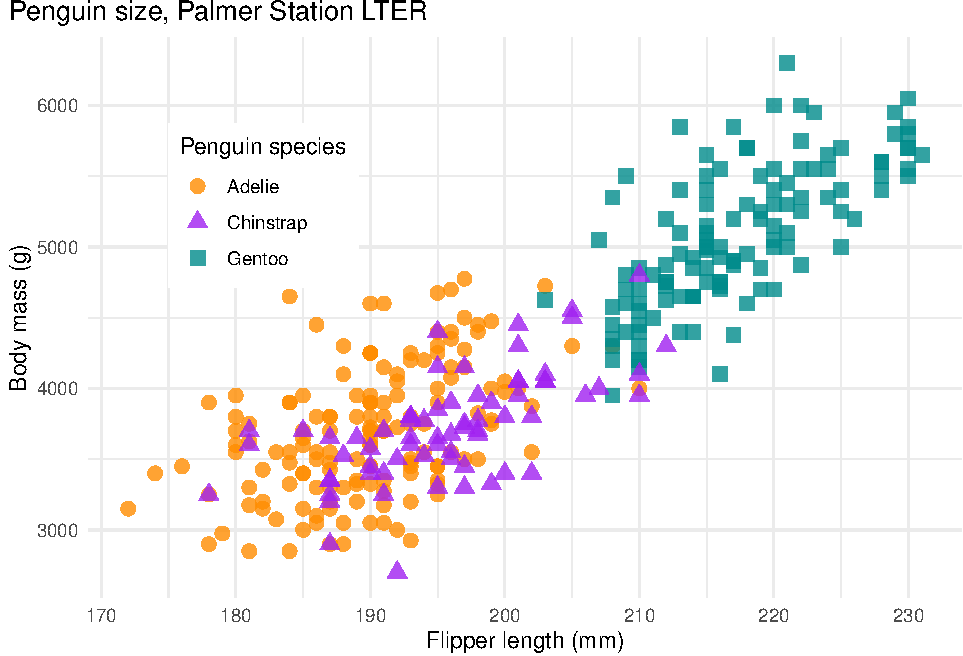
\includegraphics[width=1\linewidth]{example_files/figure-latex/penguinimage-1} \caption{Flipper length and body mass for Adelie, Chinstrap and Gentoo Penguins.}\label{fig:penguinimage}
\end{figure}

You can also use---in \texttt{doctype:\ jou} documents---the
\texttt{\textbackslash{}begin\{figure*\}} environment of LaTeX to insert
already-generated images across both columns; the code for this follows,
but an additional image is only generated for \texttt{doctype:\ jou}.
(Note that including images in the traditional R Markdown way---with
code like \texttt{!{[}Caption{]}(path/to/image.png)}---will work as
well, but will not span two columns.)

\begin{verbatim}
\begin{figure*}
\centering
\includegraphics{example_files/figure-latex/
penguinimage.pdf}
\caption{Caption for image.}
\end{figure*}
\end{verbatim}

\begin{figure*}
\centering
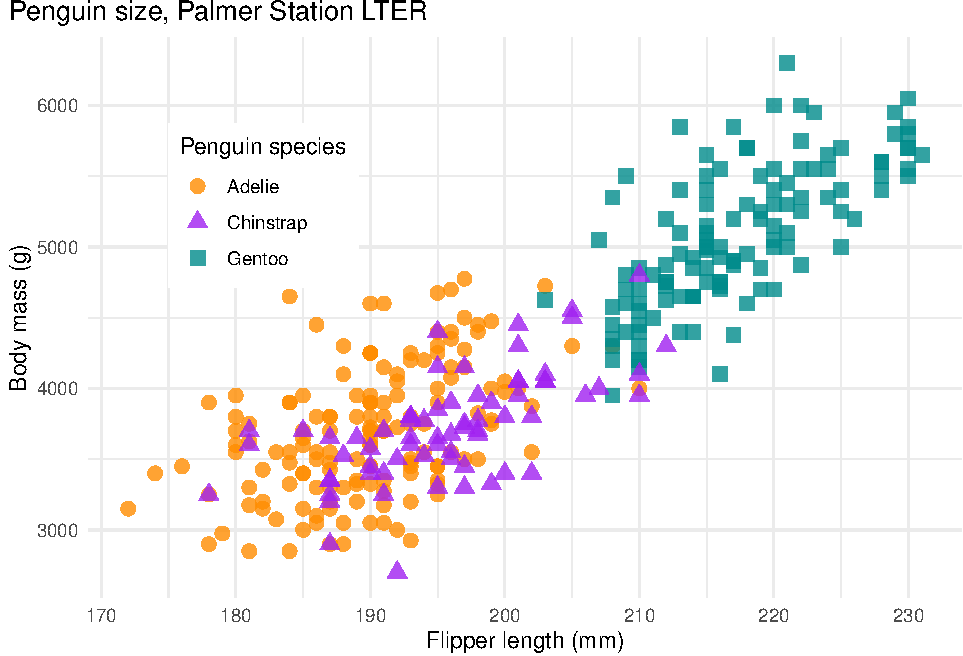
\includegraphics{example_files/figure-latex/penguinimage.pdf}
\caption{When included as an external file, images can be placed in \textbackslash{}begin\{figure*\} environments \textbackslash{}end{figure*}; these will be placed where appropriate, but will by default take up the full \textbackslash{}textwidth.}
\end{figure*}

\hypertarget{multiple-figures}{%
\subsection{Multiple figures}\label{multiple-figures}}

You can even include multiple figures concurrently in one section using
some tricks of R Markdown
\href{https://bookdown.org/yihui/rmarkdown-cookbook/latex-subfigure.html\#latex-subfigure}{as
described here}; this is why it calls
\texttt{extra\_dependencies:\ "subfig"} in the YAML at the top. However,
again, this will look relatively strange in \texttt{doctype:\ jou},
given that the images will not by default span both columns.

\begin{figure}

{\centering \subfloat[Penguin bill length negatively correlates with penguin bill depth\label{fig:morepenguins-1}]{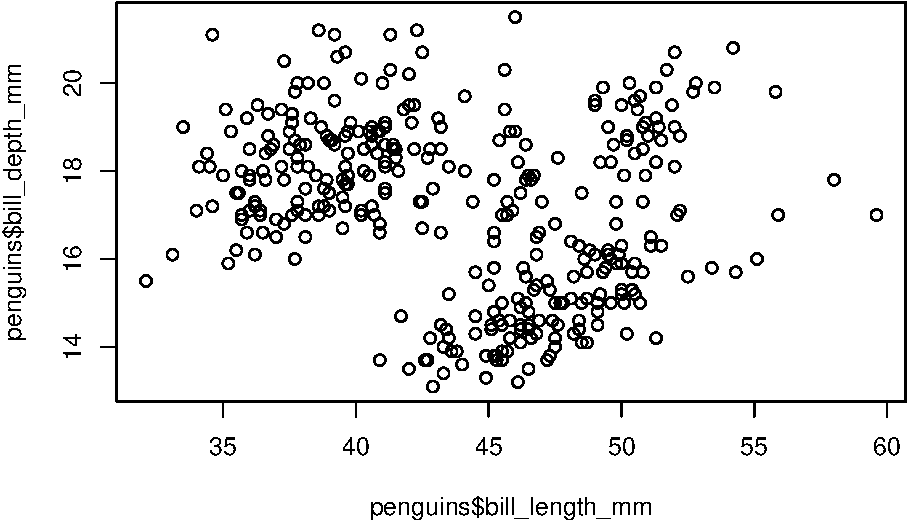
\includegraphics[width=0.5\linewidth]{example_files/figure-latex/morepenguins-1} }\subfloat[Penguin bill length positively correlates with body mass\label{fig:morepenguins-2}]{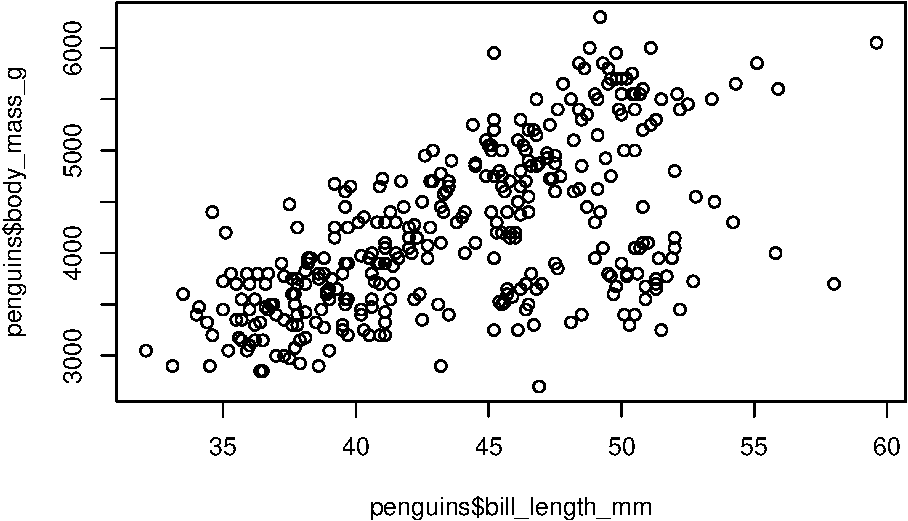
\includegraphics[width=0.5\linewidth]{example_files/figure-latex/morepenguins-2} }\newline\subfloat[Boxplot of penguin bill lengths by species\label{fig:morepenguins-3}]{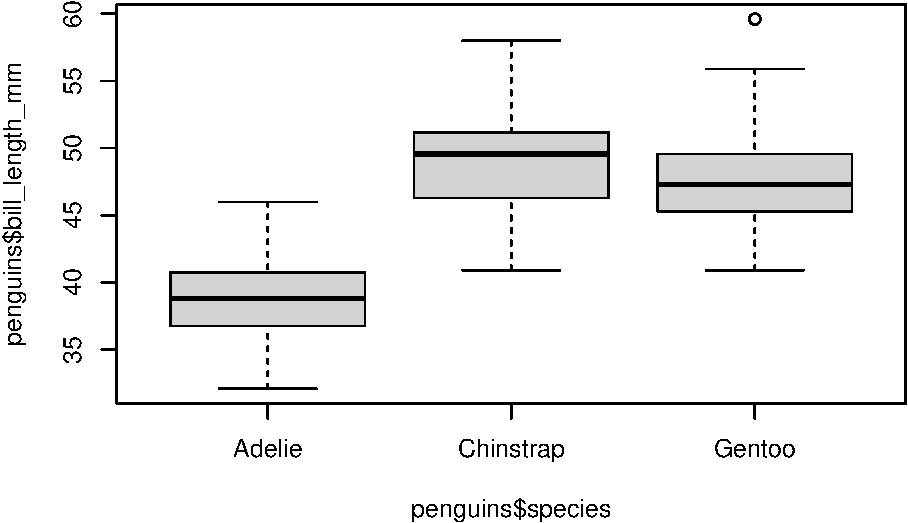
\includegraphics[width=0.5\linewidth]{example_files/figure-latex/morepenguins-3} }

}

\caption{Different ways of looking at penguin bills. Note that this sort of multiple-figure-in-one-section plot will look best in doctypes man, doc, and stu -- and be a bit abbreviated in doctype jou.}\label{fig:morepenguins}
\end{figure}

\hypertarget{including-tables}{%
\section{Including tables}\label{including-tables}}

There are many great R packages for writing LaTeX tables in R; I won't
cover them extensively here, but they include \{\emph{kableExtra}\},
\{\emph{xtable}\},
\{\emph{\href{https://gt.rstudio.com/index.html}{gt}}\},
\{\emph{\href{https://www.danieldsjoberg.com/gtsummary/}{gtsummary}}\},
and \{\emph{stargazer}\}. Most of them don't automatically format their
contents in APA style. This is one of the places where
\{\emph{\href{https://github.com/crsh/papaja}{papja}}\}, mentioned
above, can be helpful; the R functions do indeed have some intentional
formatting like \texttt{papaja::apa\_table()} which will automatically
format things \emph{for LaTeX and in APA style}. See the document
\texttt{tables\_ex.Rmd} for more.

A simple example table is included here using the
\texttt{knitr::kable()} function. Including the \texttt{caption}
argument is required for the LaTeX \{\emph{apa7}\} package to recognize
it as a table and mark it with the heading ``Table 1.''

\begin{verbatim}
library(dplyr)
penguins %>%
  group_by(island, species) %>%
  summarize(
    n = n(), 
    meanlength = mean(
      flipper_length_mm, 
      na.rm = TRUE), 
    sd = sd(flipper_length_mm, 
            na.rm = TRUE), 
    .groups = "drop"
  ) %>%
  knitr::kable(format = "latex",
  booktabs = TRUE,
  escape = FALSE,
  longtable = FALSE,
  digits = 2,
  col.names = c("Island", 
                "Species", "\\textit{n}", 
                "Flipper length (\\textit{M})", 
                "(\\textit{SD})"),
  align = c("l", "l", "c", "c", "c"),
  caption = "Summary of flipper lengths 
             across species and islands.")
\end{verbatim}

\begin{table}

\caption{\label{tab:unnamed-chunk-3}Summary of flipper lengths across species and islands.}
\centering
\begin{tabular}[t]{llccc}
\toprule
Island & Species & \textit{n} & Flipper length (\textit{M}) & (\textit{SD})\\
\midrule
Biscoe & Adelie & 44 & 188.80 & 6.73\\
Biscoe & Gentoo & 124 & 217.19 & 6.48\\
Dream & Adelie & 56 & 189.73 & 6.59\\
Dream & Chinstrap & 68 & 195.82 & 7.13\\
Torgersen & Adelie & 52 & 191.20 & 6.23\\
\bottomrule
\end{tabular}
\end{table}

\hypertarget{more-information}{%
\section{More information}\label{more-information}}

The reader hoping for more information should review some of the
following books:

\begin{itemize}
\tightlist
\item
  \href{https://bookdown.org/yihui/rmarkdown/}{R Markdown: The
  Definitive Guide} by Yihui Xie, J. J. Allaire, Garrett Grolemund
\item
  \href{https://bookdown.org/yihui/rmarkdown-cookbook/}{R Markdown
  Cookbook} by Yihui Xie, Christophe Dervieux, \& Emily Riederer
\item
  \href{https://bookdown.org/yihui/bookdown/}{bookdown: Authoring Books
  and Technical Documents with R Markdown} by Yihui Xie
\end{itemize}

\hypertarget{wrapping-up}{%
\section{Wrapping up}\label{wrapping-up}}

You needn't write anything below the title of your references
section---the bibliography will be automatically generated. If you
notice that something is inappropriately not capitalized, make sure it
is capitalized correctly in your .bib file; if it is, consider
surrounding it with curly brackets to ensure the correct formatting.

\hypertarget{references}{%
\section*{References}\label{references}}
\addcontentsline{toc}{section}{References}

\hypertarget{refs}{}
\begin{CSLReferences}{1}{0}
\leavevmode\hypertarget{ref-austbarth2020}{}%
Aust, F., \& Barth, M. (2020). \emph{{papaja}: {Create} {APA}
manuscripts with {R Markdown}}. \url{https://github.com/crsh/papaja}

\leavevmode\hypertarget{ref-weiss2021}{}%
Beitzel, B. D. (2021). \emph{Formatting documents in {APA} style (7th
{E}dition) with the apa7 LaTeX class}.
\url{http://ctan.math.washington.edu/tex-archive/macros/latex/contrib/apa7/apa7.pdf}

\leavevmode\hypertarget{ref-horst2020}{}%
Horst, A. M., Hill, A. P., \& Gorman, K. B. (2020).
\emph{{palmerpenguins}: {P}almer {A}rchipelago ({A}ntarctica) penguin
data}. \url{https://allisonhorst.github.io/palmerpenguins/}

\leavevmode\hypertarget{ref-wickham2016}{}%
Wickham, H. (2016). \emph{ggplot2: Elegant graphics for data analysis}.
Springer-Verlag New York. \url{https://ggplot2.tidyverse.org}

\leavevmode\hypertarget{ref-xie2019}{}%
Xie, Y. (2019). TinyTeX: A lightweight, cross-platform, and
easy-to-maintain LaTeX distribution based on TeX live. \emph{TUGboat},
\emph{1}, 30--32.
\url{http://tug.org/TUGboat/Contents/contents40-1.html}

\end{CSLReferences}

\end{document}